\section[Renderings]{\hl{Renderings}}
\todoa{Fix title of renderings section}
We have made some renderings of the systems we have studied, as can be seen in \crefrange{fig:renderings_rough_fracture01_abel}{fig:renderings_flat_fractures}\todoao{Check that this range is correct before handing in}. All renderings and visualizations were made using the program Ovito\cite{stukowski2010ovito}, using the built-in open-source ``Tachyon'' rendering engine.

In the renderings in this section we generally have colored the silicon atoms yellow, the oxygen atoms blue, and the hydrogen atoms white. The silicon atoms have been given a radius of 1 \AA, the oxygen atoms 0.6 \AA, and the hydrogen atoms 0.3 \AA.
%
\begin{figure}[htpb]%
    \centering%
    \setlength{\myfigwidth}{0.49\textwidth}%
%     \setlength{\mycaptionwidth}{0.3\textwidth}%
%
    \begin{subfigure}[b]{\myfigwidth}%
        \centering% % Need to center to get image centered over caption
        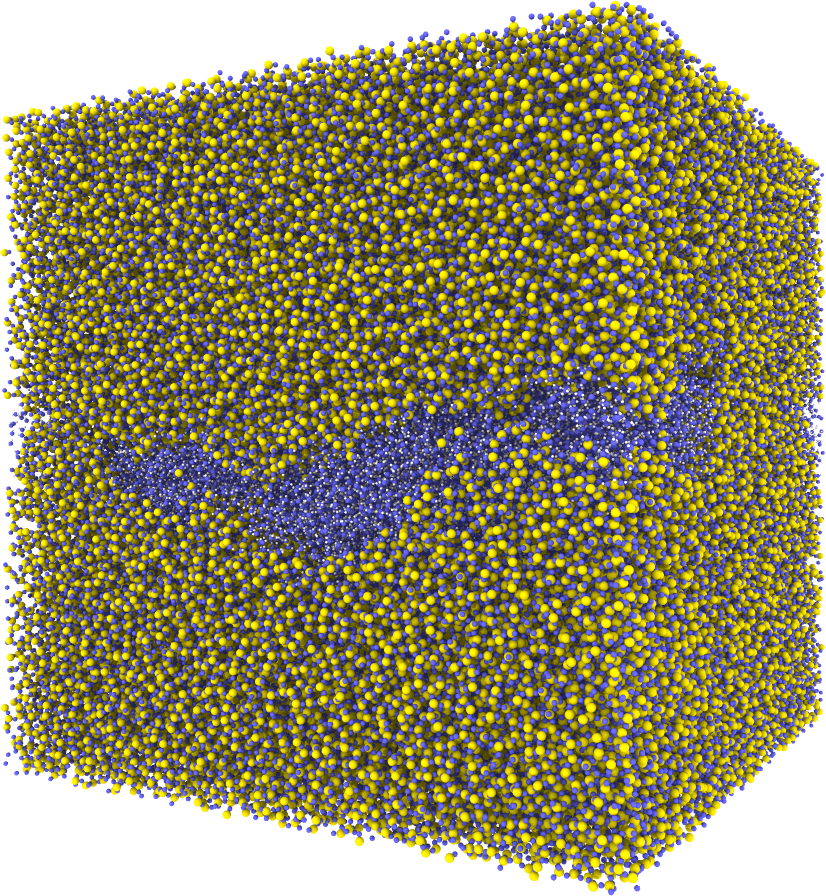
\includegraphics[width=\textwidth]{images/systems/trimmed-rough_fracture01_abel_13}%
        \caption{Caption.}%
%         \label{fig:hex_to_tetra}%
    \end{subfigure}%
    \hfill%
        \begin{subfigure}[b]{\myfigwidth}%
        \centering% % Need to center to get image centered over caption
        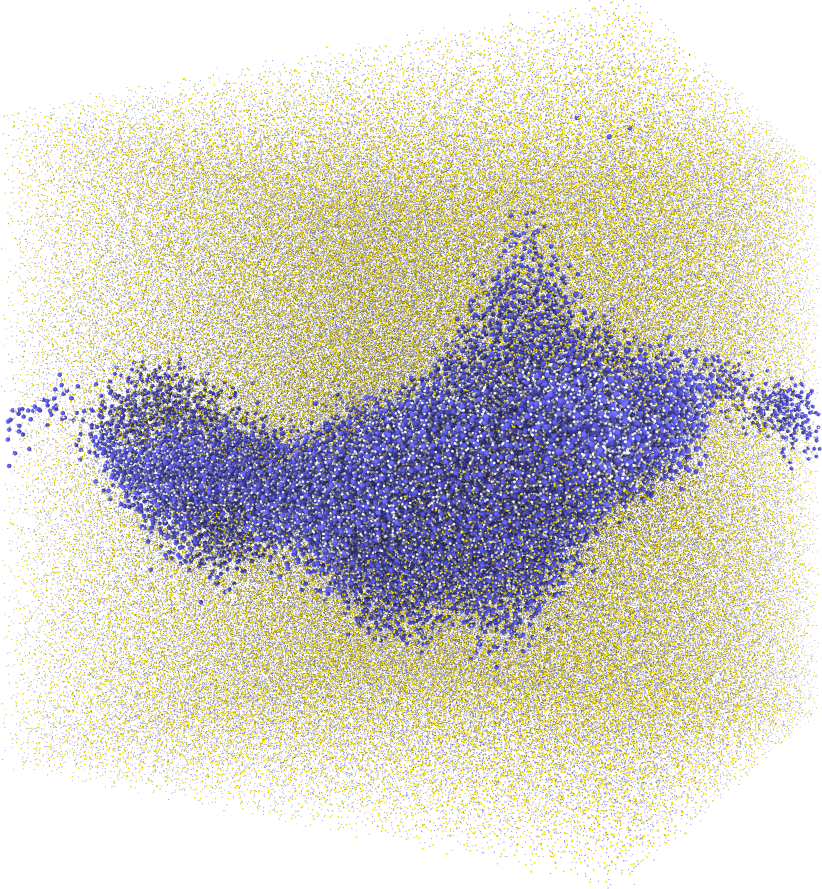
\includegraphics[width=\textwidth]{images/systems/trimmed-rough_fracture01_abel_15}%
        \caption{Caption.}%
%         \label{fig:hex_to_tetra}%
    \end{subfigure}%
    \\%
    \begin{subfigure}[b]{\myfigwidth}%
        \centering% % Need to center to get image centered over caption
        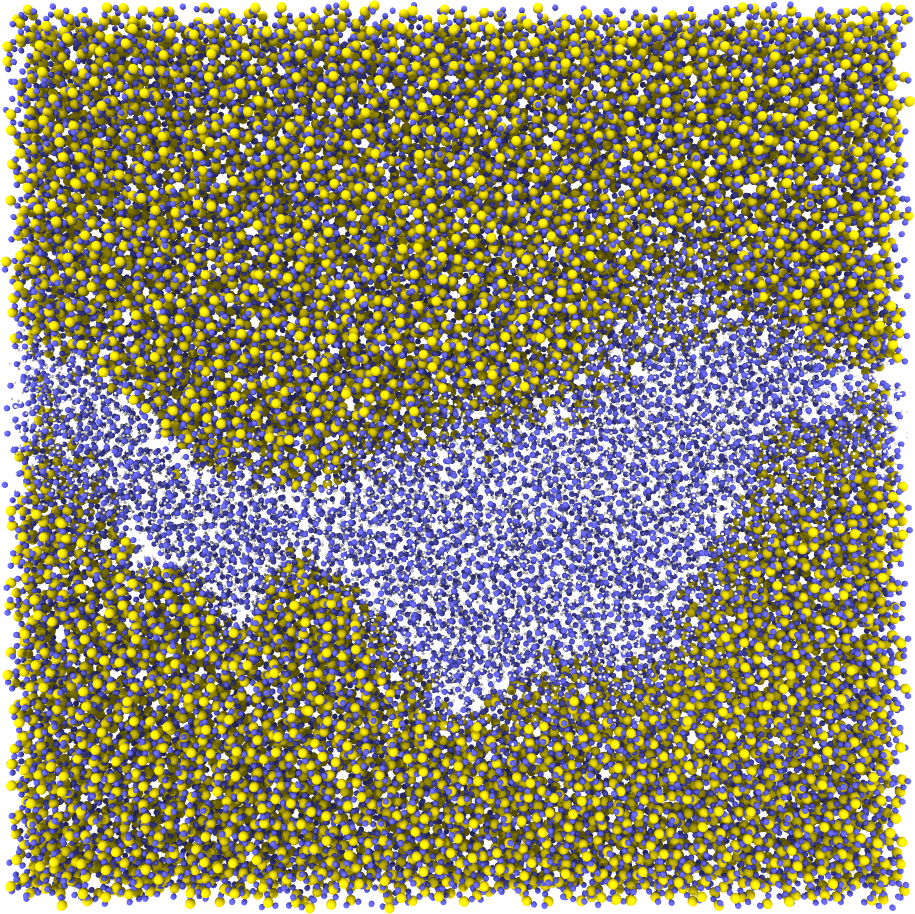
\includegraphics[width=\textwidth]{images/systems/trimmed-rough_fracture01_abel_16}%
        \caption{Caption.}%
%         \label{fig:hex_to_tetra}%
    \end{subfigure}%
    \hfill%
    \begin{subfigure}[b]{\myfigwidth}%
        \centering% % Need to center to get image centered over caption
        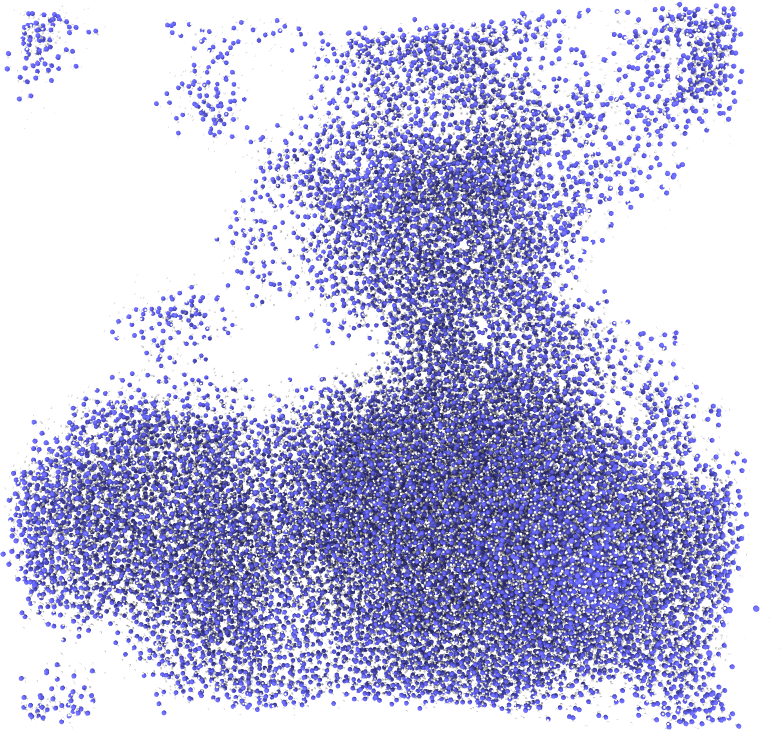
\includegraphics[width=\textwidth]{images/systems/trimmed-rough_fracture01_abel_17}%
        \caption{Caption.}%
%         \label{fig:hex_to_tetra}%
    \end{subfigure}%
    \caption{%
        rough\_fracture\_01\_abel - ``Rough fracture \#1'' \hl{Caption} %
        \label{fig:renderings_rough_fracture01_abel}%
    }%
\end{figure}%

%
\begin{figure}[htpb]%
    \centering%
    \setlength{\myfigwidth}{0.49\textwidth}%
%     \setlength{\mycaptionwidth}{0.3\textwidth}%
%
    \begin{subfigure}[b]{\myfigwidth}%
        \centering% % Need to center to get image centered over caption
        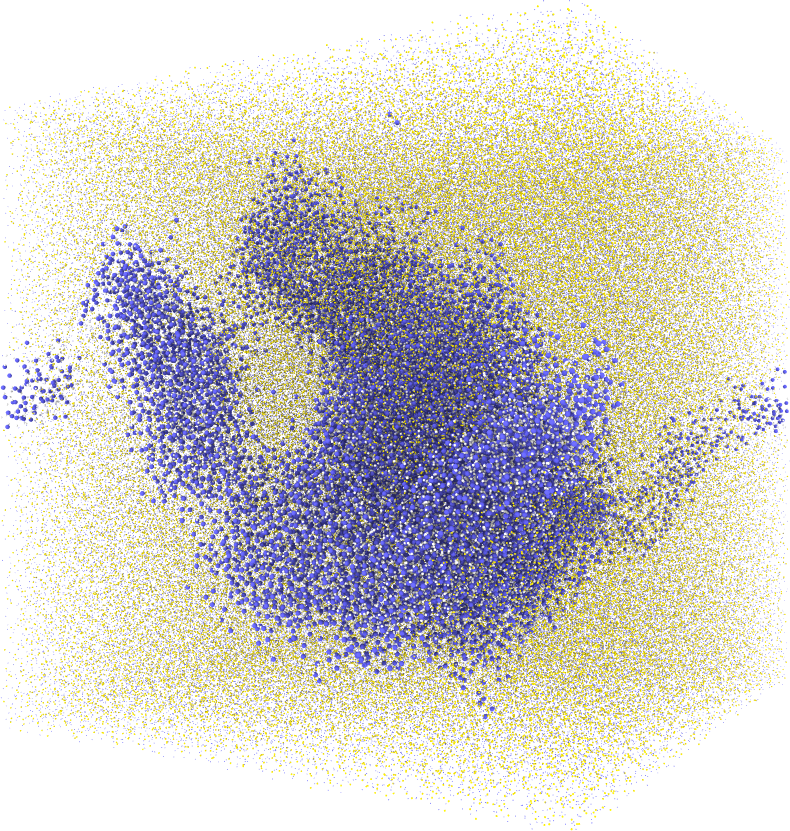
\includegraphics[width=\textwidth]{images/systems/trimmed-rough_fracture03_05}%
        \caption{Caption.}%
%         \label{fig:hex_to_tetra}%
    \end{subfigure}%
    \hfill%
    \begin{subfigure}[b]{\myfigwidth}%
        \centering% % Need to center to get image centered over caption
        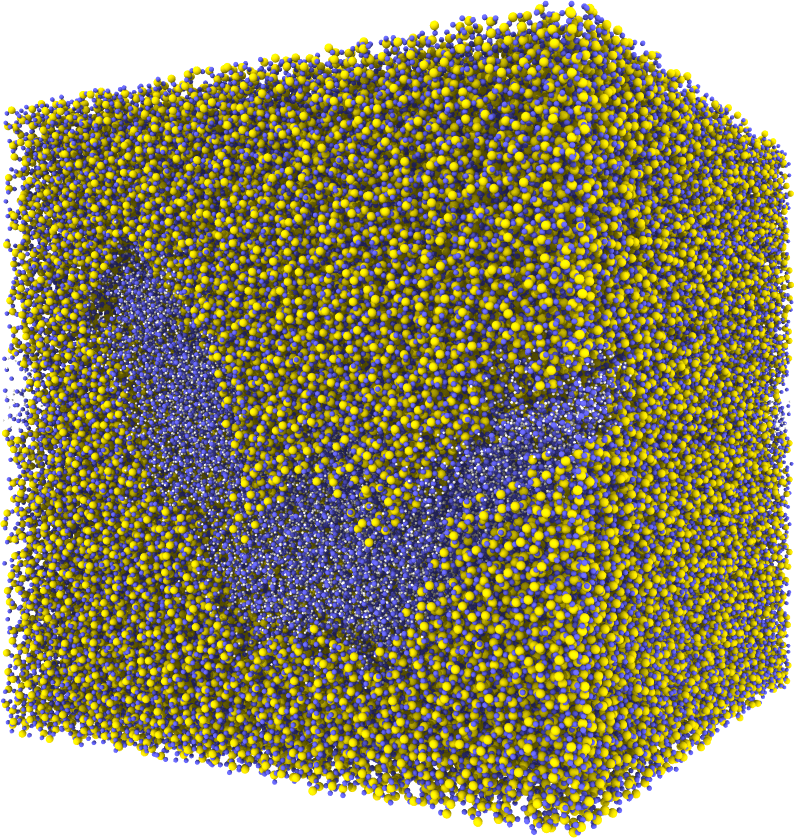
\includegraphics[width=\textwidth]{images/systems/trimmed-rough_fracture03_06}%
        \caption{Caption.}%
%         \label{fig:hex_to_tetra}%
    \end{subfigure}%
    \\%
    \begin{subfigure}[b]{\myfigwidth}%
        \centering% % Need to center to get image centered over caption
        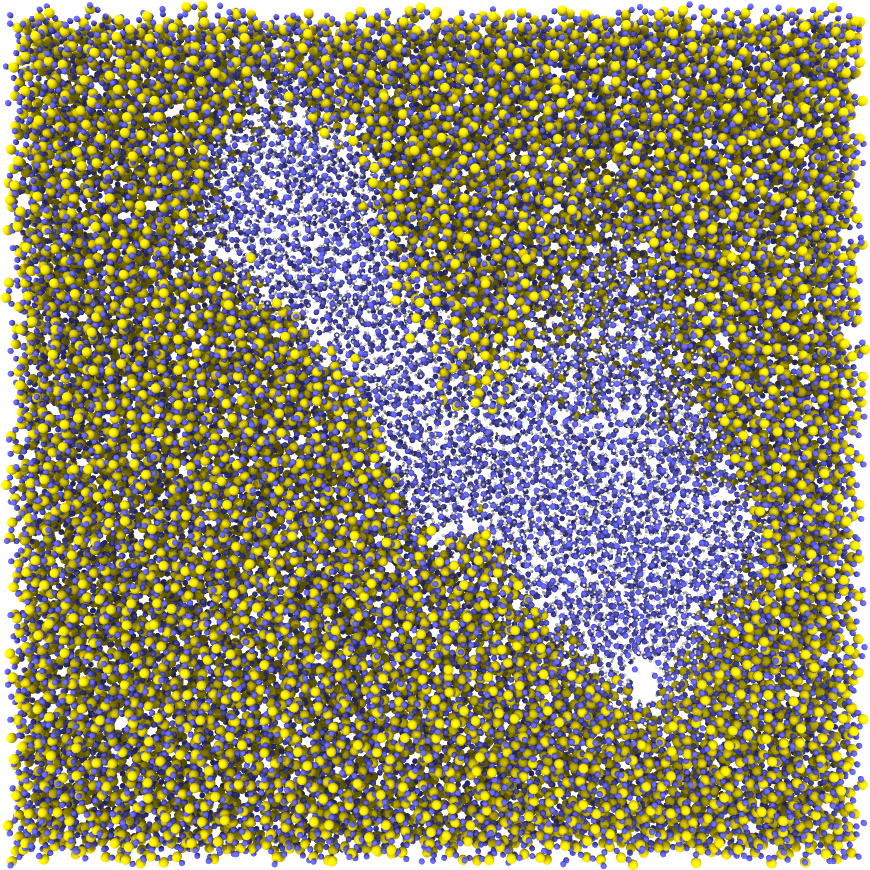
\includegraphics[width=\textwidth]{images/systems/trimmed-rough_fracture03_07}%
        \caption{Caption.}%
%         \label{fig:hex_to_tetra}%
    \end{subfigure}%
    \hfill%
    \begin{subfigure}[b]{\myfigwidth}%
        \centering% % Need to center to get image centered over caption
        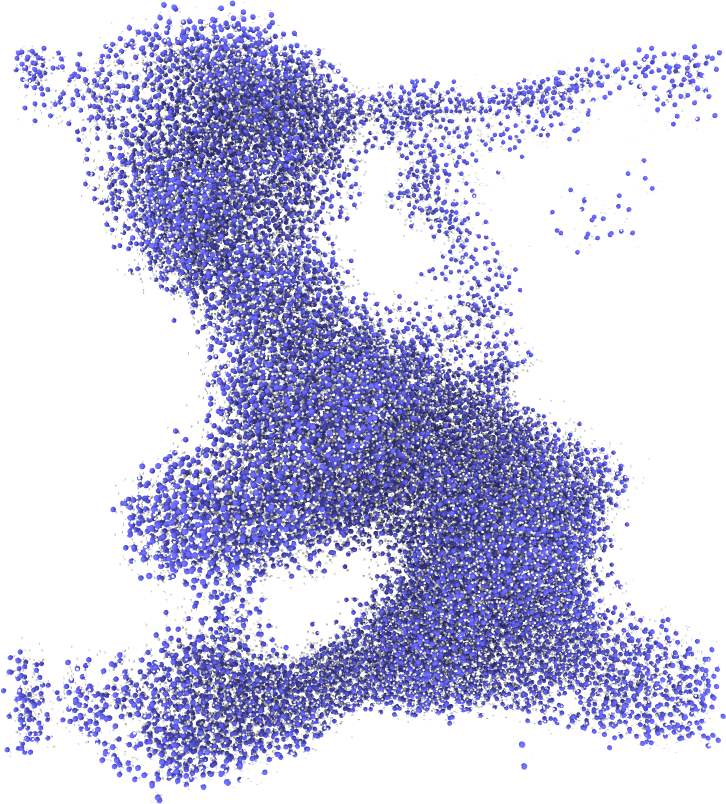
\includegraphics[width=\textwidth]{images/systems/trimmed-rough_fracture03_08}%
        \caption{Caption.}%
%         \label{fig:hex_to_tetra}%
    \end{subfigure}%
    \caption{%
        rough\_fracture\_03 - ``Rough fracture \#2'' \hl{Caption} %
        \label{fig:renderings_rough_fracture03}%
    }%
\end{figure}%

%
\begin{figure}[htpb]%
    \centering%
    \setlength{\myfigwidth}{0.49\textwidth}%
%     \setlength{\mycaptionwidth}{0.3\textwidth}%
%
    \begin{subfigure}[b]{\myfigwidth}%
        \centering% % Need to center to get image centered over caption
        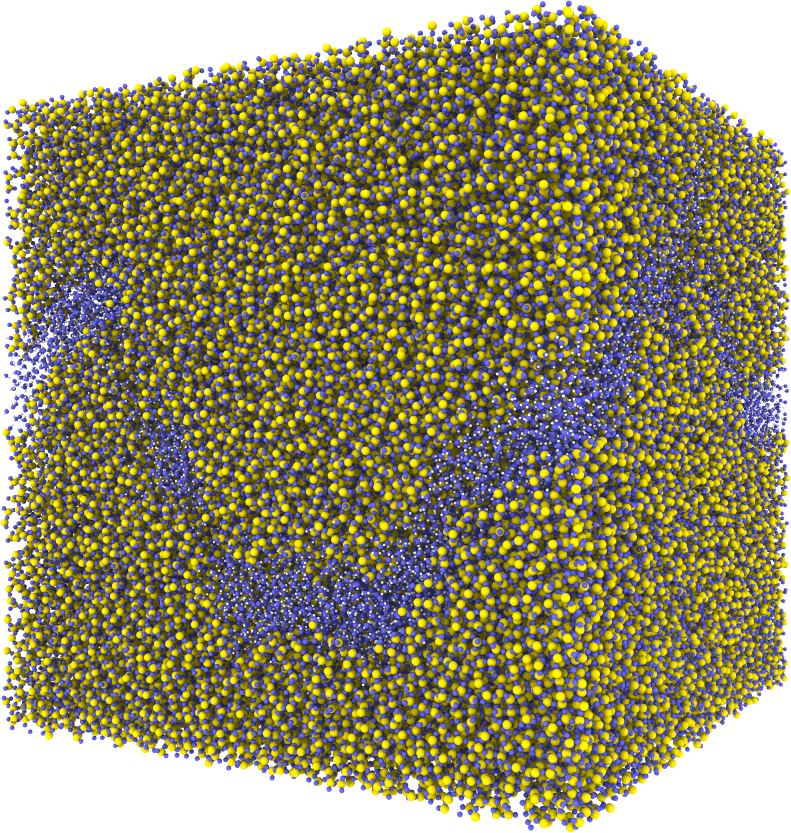
\includegraphics[width=\textwidth]{images/systems/trimmed-rough_fracture04_06}%
        \caption{Caption.}%
%         \label{fig:hex_to_tetra}%
    \end{subfigure}%
    \hfill%
    \begin{subfigure}[b]{\myfigwidth}%
        \centering% % Need to center to get image centered over caption
        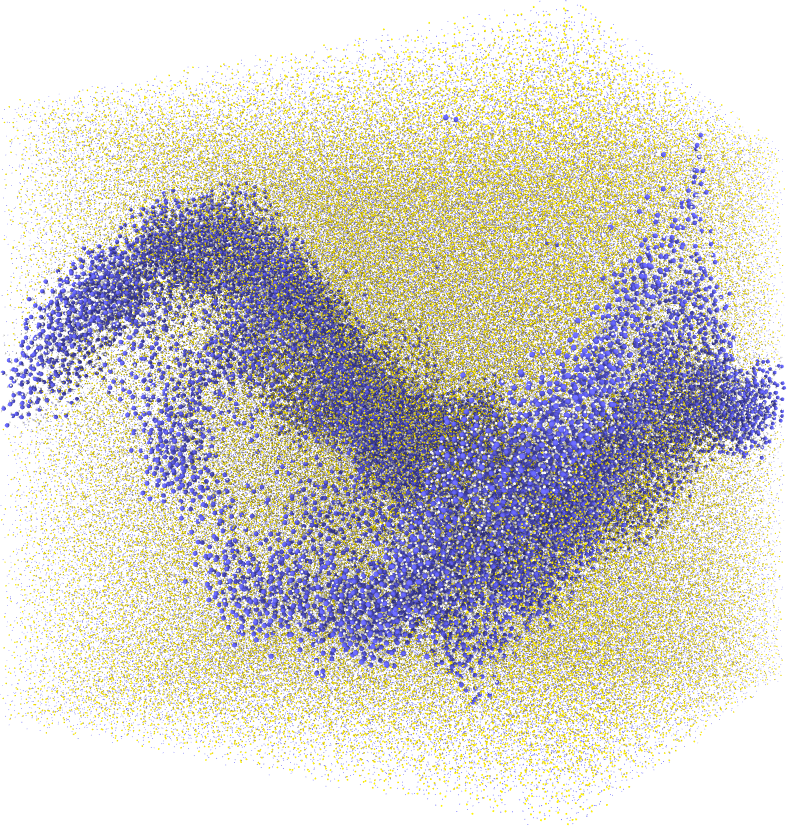
\includegraphics[width=\textwidth]{images/systems/trimmed-rough_fracture04_07}%
        \caption{Caption.}%
%         \label{fig:hex_to_tetra}%
    \end{subfigure}%
    \\%
    \begin{subfigure}[b]{\myfigwidth}%
        \centering% % Need to center to get image centered over caption
        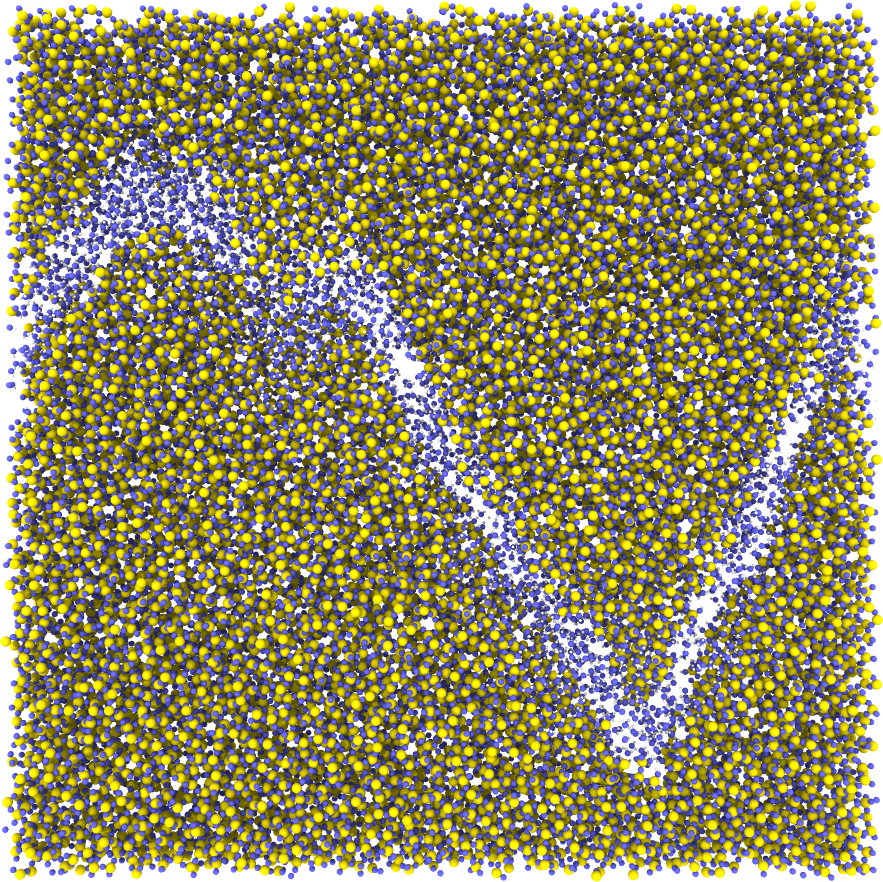
\includegraphics[width=\textwidth]{images/systems/trimmed-rough_fracture04_05_20ang}%
        \caption{Caption.}%
%         \label{fig:hex_to_tetra}%
    \end{subfigure}%
    \hfill%
    \begin{subfigure}[b]{\myfigwidth}%
        \centering% % Need to center to get image centered over caption
        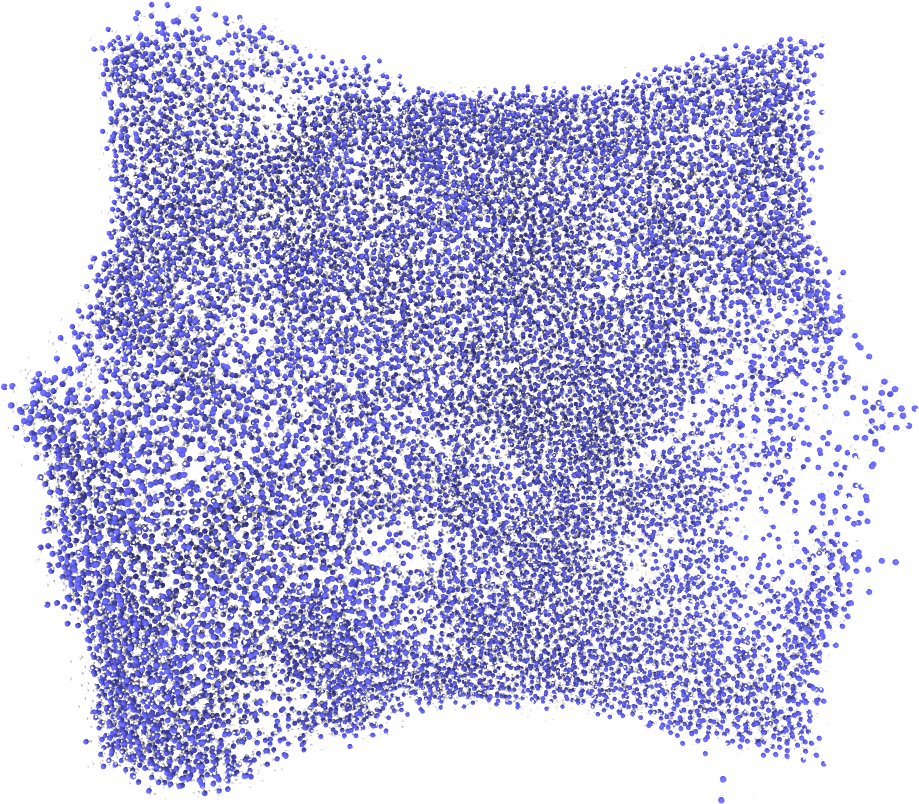
\includegraphics[width=\textwidth]{images/systems/trimmed-rough_fracture04_08}%
        \caption{Caption.}%
%         \label{fig:hex_to_tetra}%
    \end{subfigure}%
    \caption{%
        rough\_fracture\_04\_same\_distance - ``Rough fracture \#3'' \hl{Caption} %
        \label{fig:renderings_rough_fracture04_same_distance}%
    }%
\end{figure}%

%
\begin{figure}[htpb]%
    \centering%
    \setlength{\myfigwidth}{0.49\textwidth}%
%     \setlength{\mycaptionwidth}{0.3\textwidth}%
%
    \begin{subfigure}[b]{\myfigwidth}%
        \centering% % Need to center to get image centered over caption
        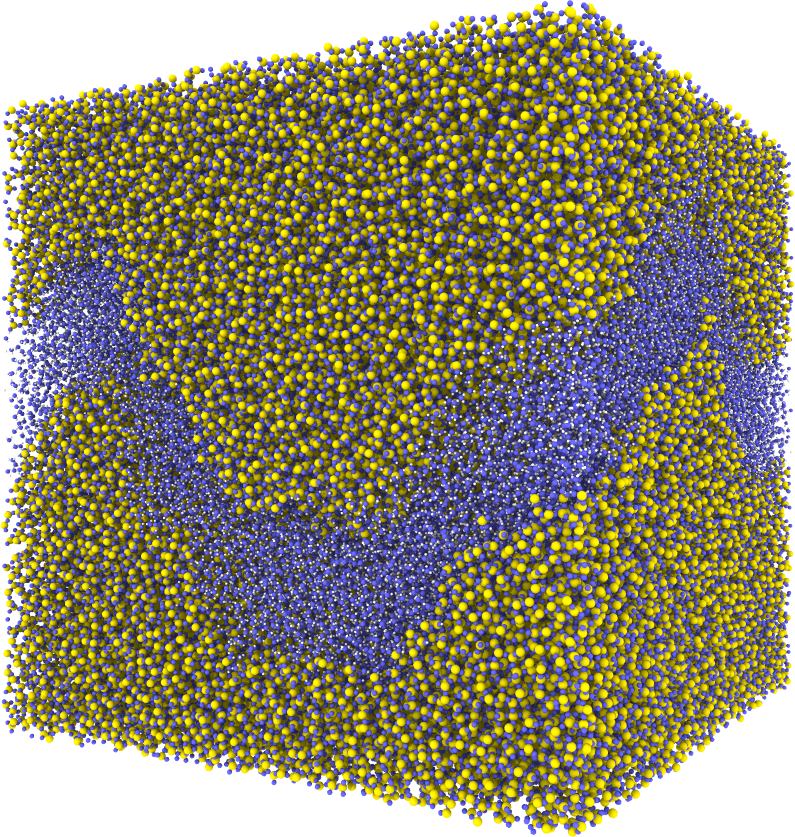
\includegraphics[width=\textwidth]{images/systems/trimmed-rough_fracture05_05}%
        \caption{Caption.}%
%         \label{fig:hex_to_tetra}%
    \end{subfigure}%
    \hfill%
    \begin{subfigure}[b]{\myfigwidth}%
        \centering% % Need to center to get image centered over caption
        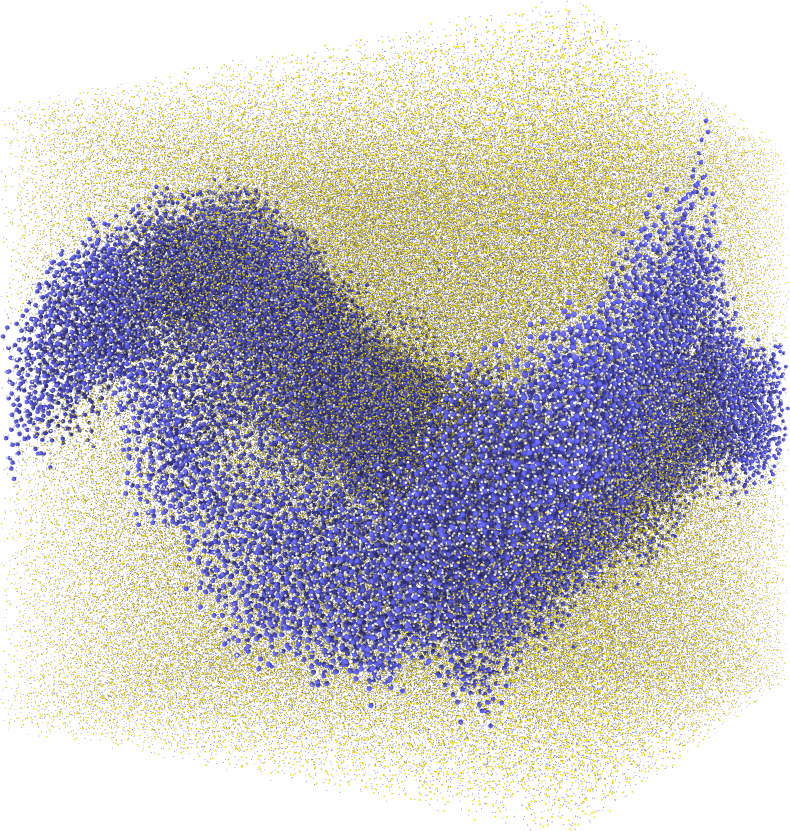
\includegraphics[width=\textwidth]{images/systems/trimmed-rough_fracture05_04}%
        \caption{Caption.}%
%         \label{fig:hex_to_tetra}%
    \end{subfigure}%
    \\%
    \begin{subfigure}[b]{\myfigwidth}%
        \centering% % Need to center to get image centered over caption
        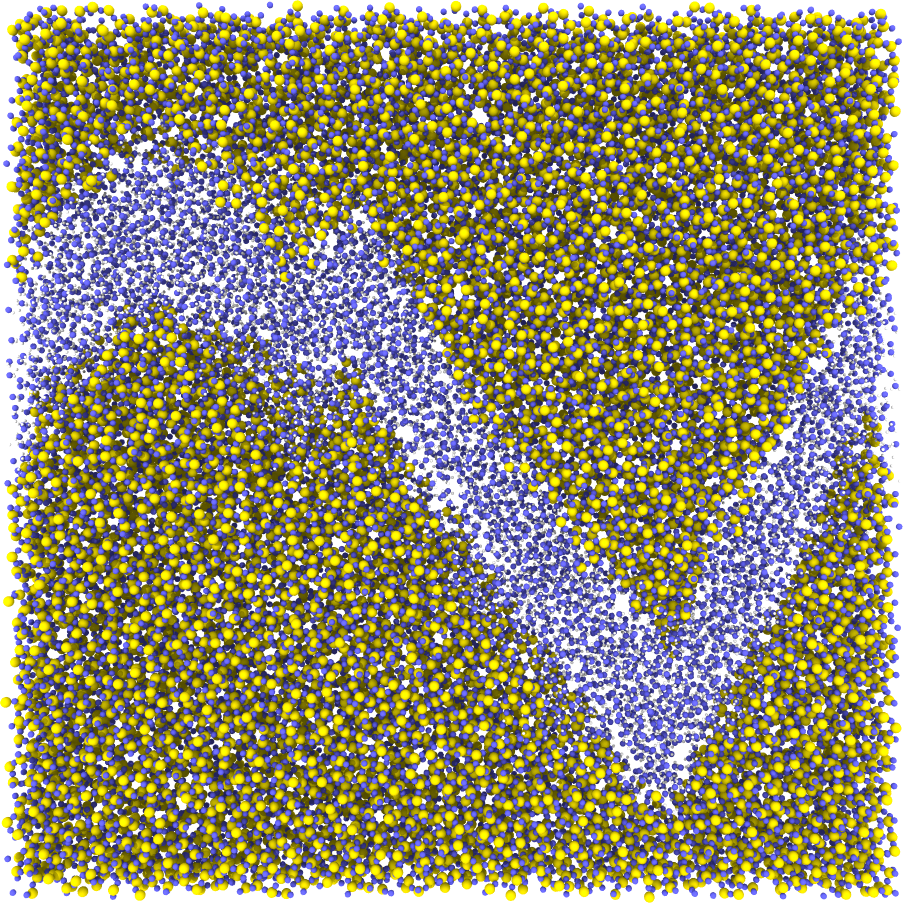
\includegraphics[width=\textwidth]{images/systems/trimmed-rough_fracture05_02_20ang}%
        \caption{Caption.}%
%         \label{fig:hex_to_tetra}%
    \end{subfigure}%
    \hfill%
    \begin{subfigure}[b]{\myfigwidth}%
        \centering% % Need to center to get image centered over caption
        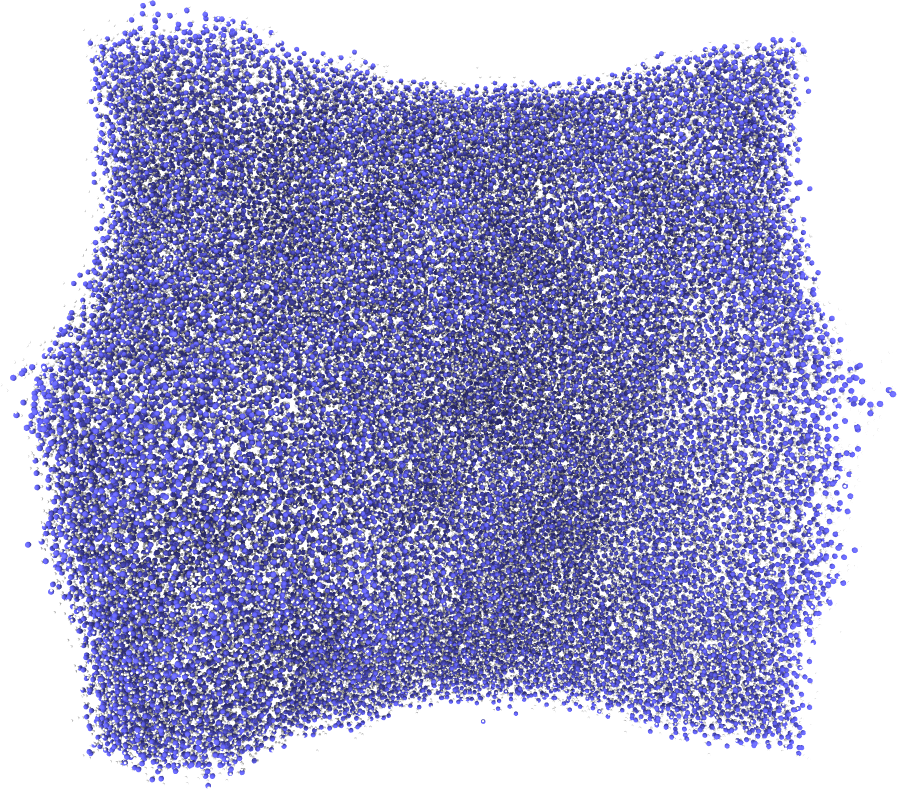
\includegraphics[width=\textwidth]{images/systems/trimmed-rough_fracture05_06}%
        \caption{Caption.}%
%         \label{fig:hex_to_tetra}%
    \end{subfigure}%
    \caption{%
        rough\_fracture\_05 - ``Rough fracture \#4'' \hl{Caption} %
        \label{fig:renderings_rough_fracture05}%
    }%
\end{figure}%

%
\begin{figure}[htpb]%
    \centering%
    \setlength{\myfigwidth}{0.49\textwidth}%
%     \setlength{\mycaptionwidth}{0.3\textwidth}%
%
    \begin{subfigure}[b]{\myfigwidth}%
        \centering% % Need to center to get image centered over caption
        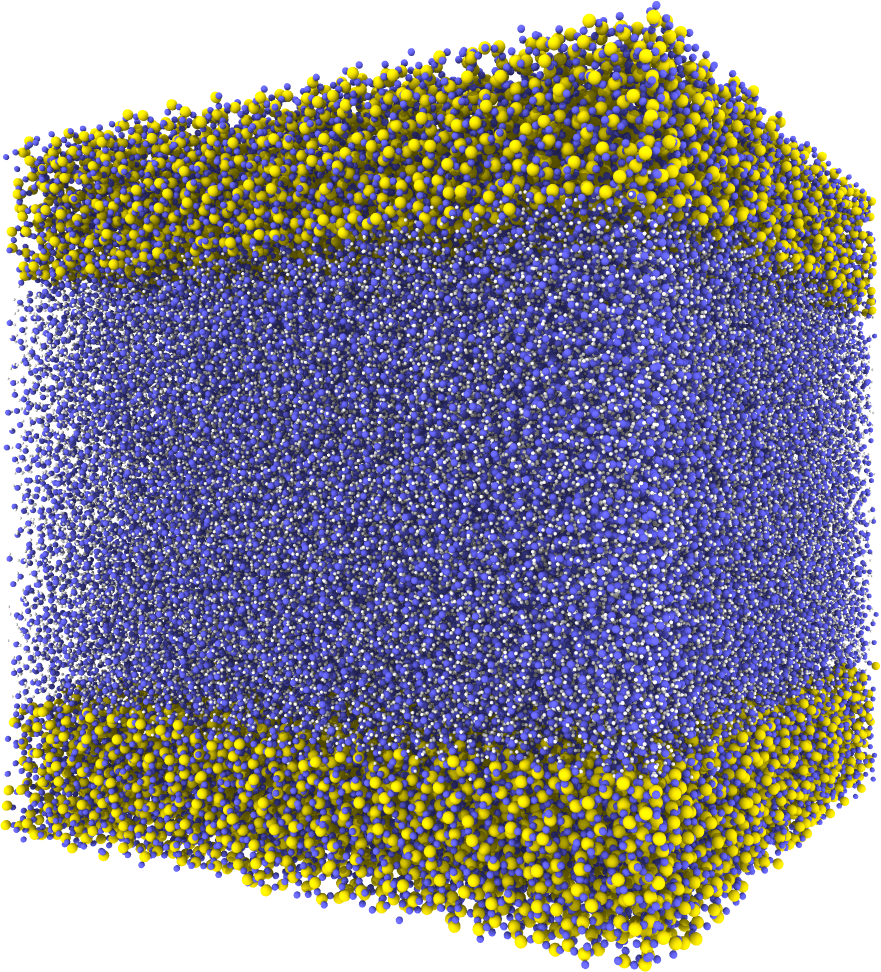
\includegraphics[width=\textwidth]{images/systems/trimmed-flat_square_fracture02_03}%
        \caption{%
            flat\_square\_fracture\_02 - ``Flat fracture \#1'' \hl{Caption} %
        }%
        \label{fig:renderings_flat_square_fracture02}%
    \end{subfigure}%
    \hfill%
    \begin{subfigure}[b]{\myfigwidth}%
        \centering% % Need to center to get image centered over caption
        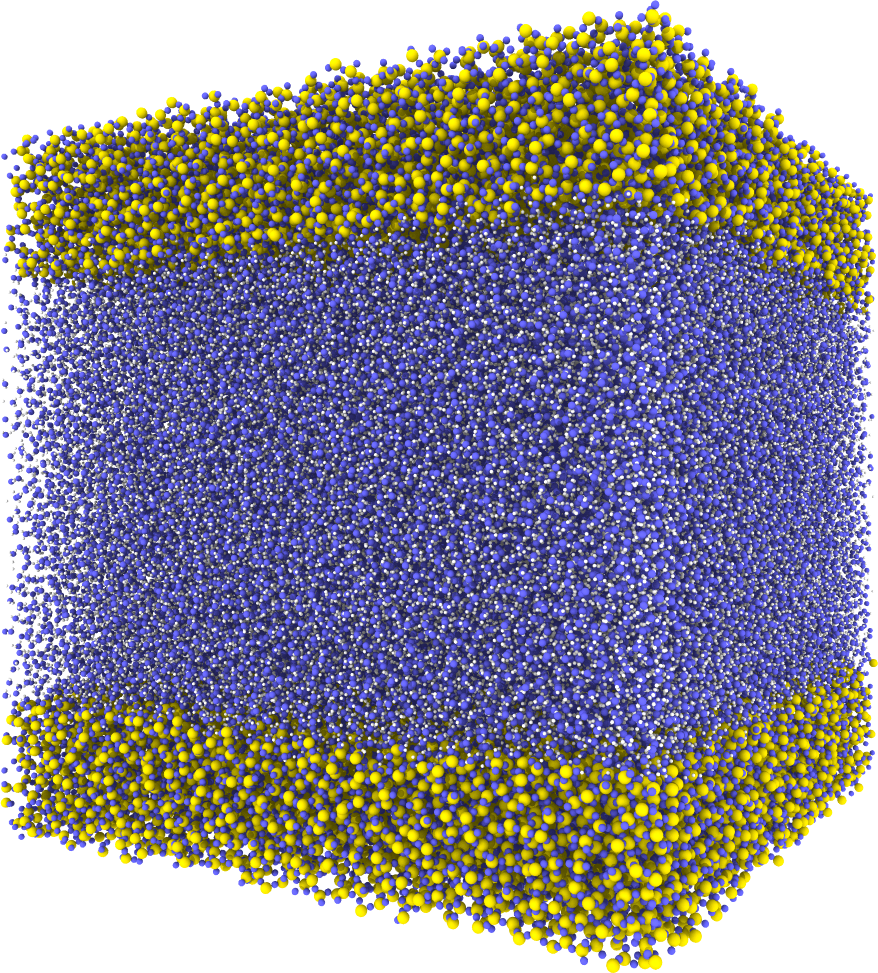
\includegraphics[width=\textwidth]{images/systems/trimmed-flat_square_fracture03_04}%
        \caption{%
            flat\_square\_fracture\_03 - ``Flat fracture \#2'' \hl{Caption} %
        }%
        \label{fig:renderings_flat_square_fracture03}%
    \end{subfigure}%
    \\%
    \begin{subfigure}[b]{\myfigwidth}%
        \centering% % Need to center to get image centered over caption
        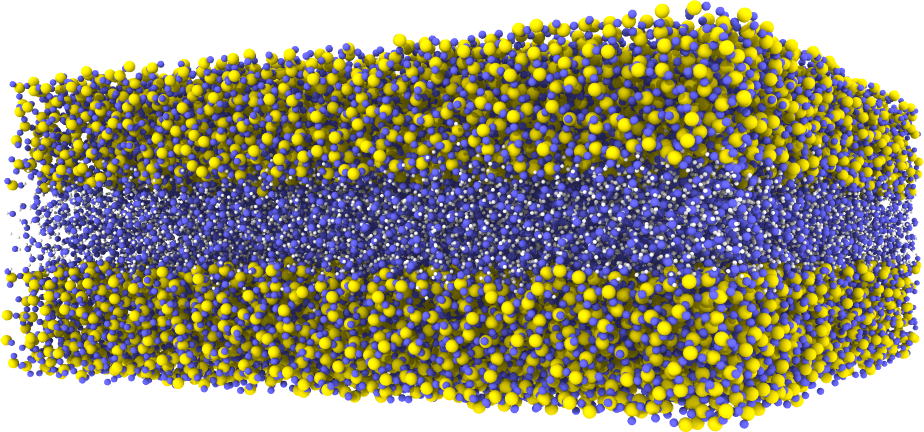
\includegraphics[width=\textwidth]{images/systems/trimmed-flat_fracture02_03}%
        \caption{%
            flat\_fracture\_02 - ``Flat fracture \#3'' \hl{Caption} %
        }%
        \label{fig:renderings_flat_fracture02}%
    \end{subfigure}%
    \hfill%
    \begin{subfigure}[b]{\myfigwidth}%
        \centering% % Need to center to get image centered over caption
        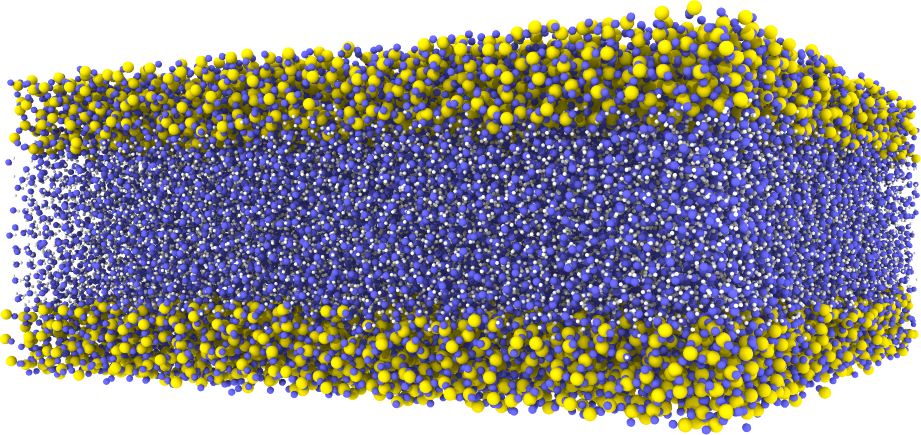
\includegraphics[width=\textwidth]{images/systems/trimmed-flat_fracture03_03}%
        \caption{%
            flat\_fracture\_03 - ``Flat fracture \#4'' \hl{Caption} %
        }%
        \label{fig:renderings_flat_fracture03}%
    \end{subfigure}%
    \caption{%
        Flat fracture \#1-4
        \label{fig:renderings_flat_fractures}%
    }%
\end{figure}%
%